\chapter{Développement de l'application}
\minitoc

\section{Intégration du moteur de reconnaissance vocale}

\subsection{Préambule}
La reconnaissance vocale de notre application s'effectue à l'aide du moteur Speechroot, développé il y a une dizaine d'années par l'entreprise IBM en langage C.
Pour des raisons de confidentialité, nous n'avons pas accès au code source de ce moteur mais à son interface nous permettant de l'exploiter.
Cette interface JNI va nous permettre d'intégrer le moteur dans notre application, écrite en Java.
Comme nous l'avons déjà signalé auparavant, ce moteur a été compilé pour Windows et ne peut donc pas être exécuté sur d'autres systèmes d'exploitation.

\subsection{Fonctionnalités du moteur}
A partir de l'interface JNI, nous avons accès à une liste de fonctionnalités que nous pouvons alors appeler.
Les fonctions de bases du moteur sont les suivantes~:
\begin{itemize}
\item démarrage et arrêt du moteur de reconnaissance vocale,
\item ouverture et fermeture du microphone,
\item ouverture de l'interface de gestion des dictionnaires,
\item ouverture de l'interface de gestion des modèles vocaux.
\end{itemize}	

Le moteur effectue ses retours à l'aide d'une fonction de callback que nous lui spécifions lors d'une initialisation obligatoire, avant son démarrage.
Cette fonction prend en paramètres deux chaînes de caractères représentant le type de message et son corps.
Les retours qui nous intéressent le plus sont donc ceux qui correspondent à résultat de la traduction effectuée par le moteur.
Ces retours sont identifiés par le type de message \texttt{onNewReco} et leur corps respecte la syntaxe~:
\begin{verbatim}
WORDS###confidence score###Pronunciation###begin word time//end word time
    ###flags
\end{verbatim}
où \texttt{WORDS} correspond aux mots reconnus et le reste aux paramètres du moteur.
Les paramètres correspondent à~:
\begin{description}
\item [\texttt{confidence score}~:] nombre compris entre -100 et 100 et qui représente au degré de confiance de la reconnaissance.
\item [\texttt{Pronunciation}~:] la prononciation des mots, similaire à l'alphabet phonétique international.
\item [\texttt{begin word time}~:] l'heure de début de la reconnaissance de ces mots.
\item [\texttt{end word time}~:] l'heure de fin de la reconnaissance de ces mots.
\item [\texttt{flags}~:] Drapeaux indiquant des informations supplémentaires telles que :
\begin{itemize}
\item le prochain mot commencera par une majuscule.
\item le prochain mot sera collé au précédent.
\item etc.
\end{itemize}
\end{description}

Le moteur offre également d'autres fonctionnalités que nous n'exploiterons pas, comme par exemple la reconnaissance vocale d'un fichier audio ou la possibilité de conserver le flux audio de la transcription.

\subsection{Intégration}
Afin que notre application soit évolutive au maximum et qu'elle ne dépende pas d'un unique moteur de reconnaissance vocale, nous avons conçu une interface disposant des fonctionnalités de base que nous avons énuméré auparavant (voir figure~\ref{fig:engineDiagram}).
Comme notre objectif est d'intégrer en particulier le moteur Speechroot, nous avons pensé cette interface de manière à ce qu'elle se calque parfaitement avec lui.

\begin{figure}[ht!]
 \centering
 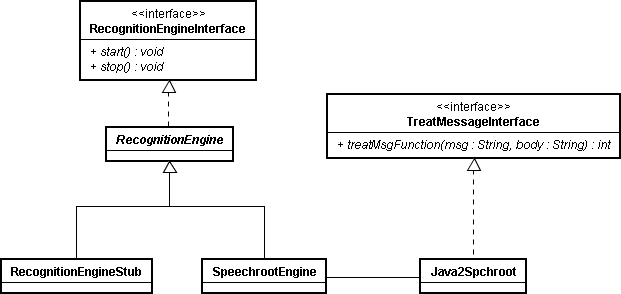
\includegraphics[scale=.5,keepaspectratio=true]{./images/EngineDiagram.png}
 % EngineDiagram.png: 621x294 pixel, 72dpi, 21.90x10.37 cm, bb=0 0 621 294
 \caption{Diagramme des classes du moteur de reconnaissance vocale}
 \label{fig:engineDiagram}
\end{figure}

La présence de la classe abstraite implémentant l'interface se justifie par le fait que le moteur est observé par le contrôleur de notre application.
Il doit en conséquent étendre la classe \texttt{java.util.Observable}, ce que nous ne pouvons pas spécifier avec seulement une interface.

Dans le cas de Speechroot, le moteur doit utiliser une classe implémentant l'interface fournie par IBM~: \texttt{TreatMessageInterface}.
Cette interface spécifie la fonction de callback qui doit être passée en paramètre lors du démarrage du moteur.
C'est donc dans l'implémentation de cette fonction que nous décodons le corps du message pour ensuite le transmettre au contrôleur à l'aide du patron de conception ``observateur''.

Nous avons rencontré quelques difficultés concernant les retours de callback du moteur Speechroot.
En effet, les retours ne s'effectuaient pas correctement~: nous ne les récupérions pas tant que nous n'exécutions pas un appel aux interfaces de gestion des dictionnaires ou des modèles vocaux.
Nous en avons déduis qu'il devait probablement y avoir un processus bloquant au sein du moteur.
Pour cette raison, nous avons écris rapidement un bouchon simulant l'action de ce moteur, afin de pouvoir poursuivre notre projet sans nous soucier de ce problème que nous ne pouvions pas régler seuls.
Puisque que tous ces moteurs étendent la même classe, et que c'est cette classe abstraite que nous appelons dans le contrôleur, il est extrêmement facile d'échanger le bouchon par le véritable moteur Speechroot, dès que le soucis de ce dernier sera réglé.
Bien que ce n'était pas notre intention originelle, nous avons préféré lors de notre soutenance faire la démonstration de notre application munie du bouchon plutôt que du moteur Speechroot pour montrer au mieux les possibilités qu'offrait notre interface graphique, cœur de notre projet.



\section{Déploiement de la base de données embarquée}

Afin de permettre l’enregistrement des cours de manière simple et intuitive, nous avons souhaité mettre en place une base de données. 
Cela permettra à l’utilisateur de classer les cours comme il le souhaite et de retrouver ces derniers rapidement, à la manière d’un client de messagerie.
Comme la base doit démarrer avec le programme, cette dernière doit être embarquée.
Nous avons choisi d’utiliser H2, base de données embarquée et légère, qui nous a été conseillée lors de notre formation.

Lors de la réalisation de cette base de données, nous avons utilisé surtout deux patrons de conception. 

Pour effectuer l’abstraction des données, l’utilisation du pattern DAO parait ici tout indiquée, cela permet de séparer les entités d'accès à la base de manière simple et fonctionnelle.
Il s'agit surtout de ne pas écrire ces accès dans les classes "métier", qui ne seront modifiées que si les règles de gestion métier changent.

Pour la conceptualisation de la base, nous avons utilisé le pattern composite.
Un objet composite est constitué d'un ou de plusieurs objets similaires (ayant des fonctionnalités similaires). 
L'idée est de manipuler un groupe d'objets de la même façon que s'il s'agissait d'un seul type d’objet, en utilisant leurs opérations communes.
Ici, nous avons voulu mettre en place des cours (fichiers) et des dossiers.
Nous en avons extrait les opérations communes et avons défini le type abstrait Element, qui devient alors classe mère des deux autres.
Une fois cela réalisé, le type dossier (Folder) peut alors référencer des éléments, sans se soucier du type final  (voir figure~\ref{fig:compositeDiagram}).

\begin{figure}[ht!]
 \centering
 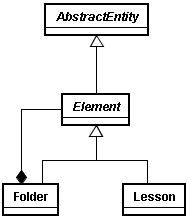
\includegraphics[scale=1,keepaspectratio=true]{./images/CompositeDiagram.png}
 \caption{Diagramme des classes de la base de données}
 \label{fig:compositeDiagram}
\end{figure}

Afin de gérer la persistance,  les classes « métiers » ont été annotées. Cela évite de faire un mappage XML pénible et potentiellement source d’erreurs.

